\chapter{Photoluminescence results on a variety of InAs/GaAsSb/GaAs samples}


\label{chapter:appendix_SciRep}
\begin{figure}
	\centering
	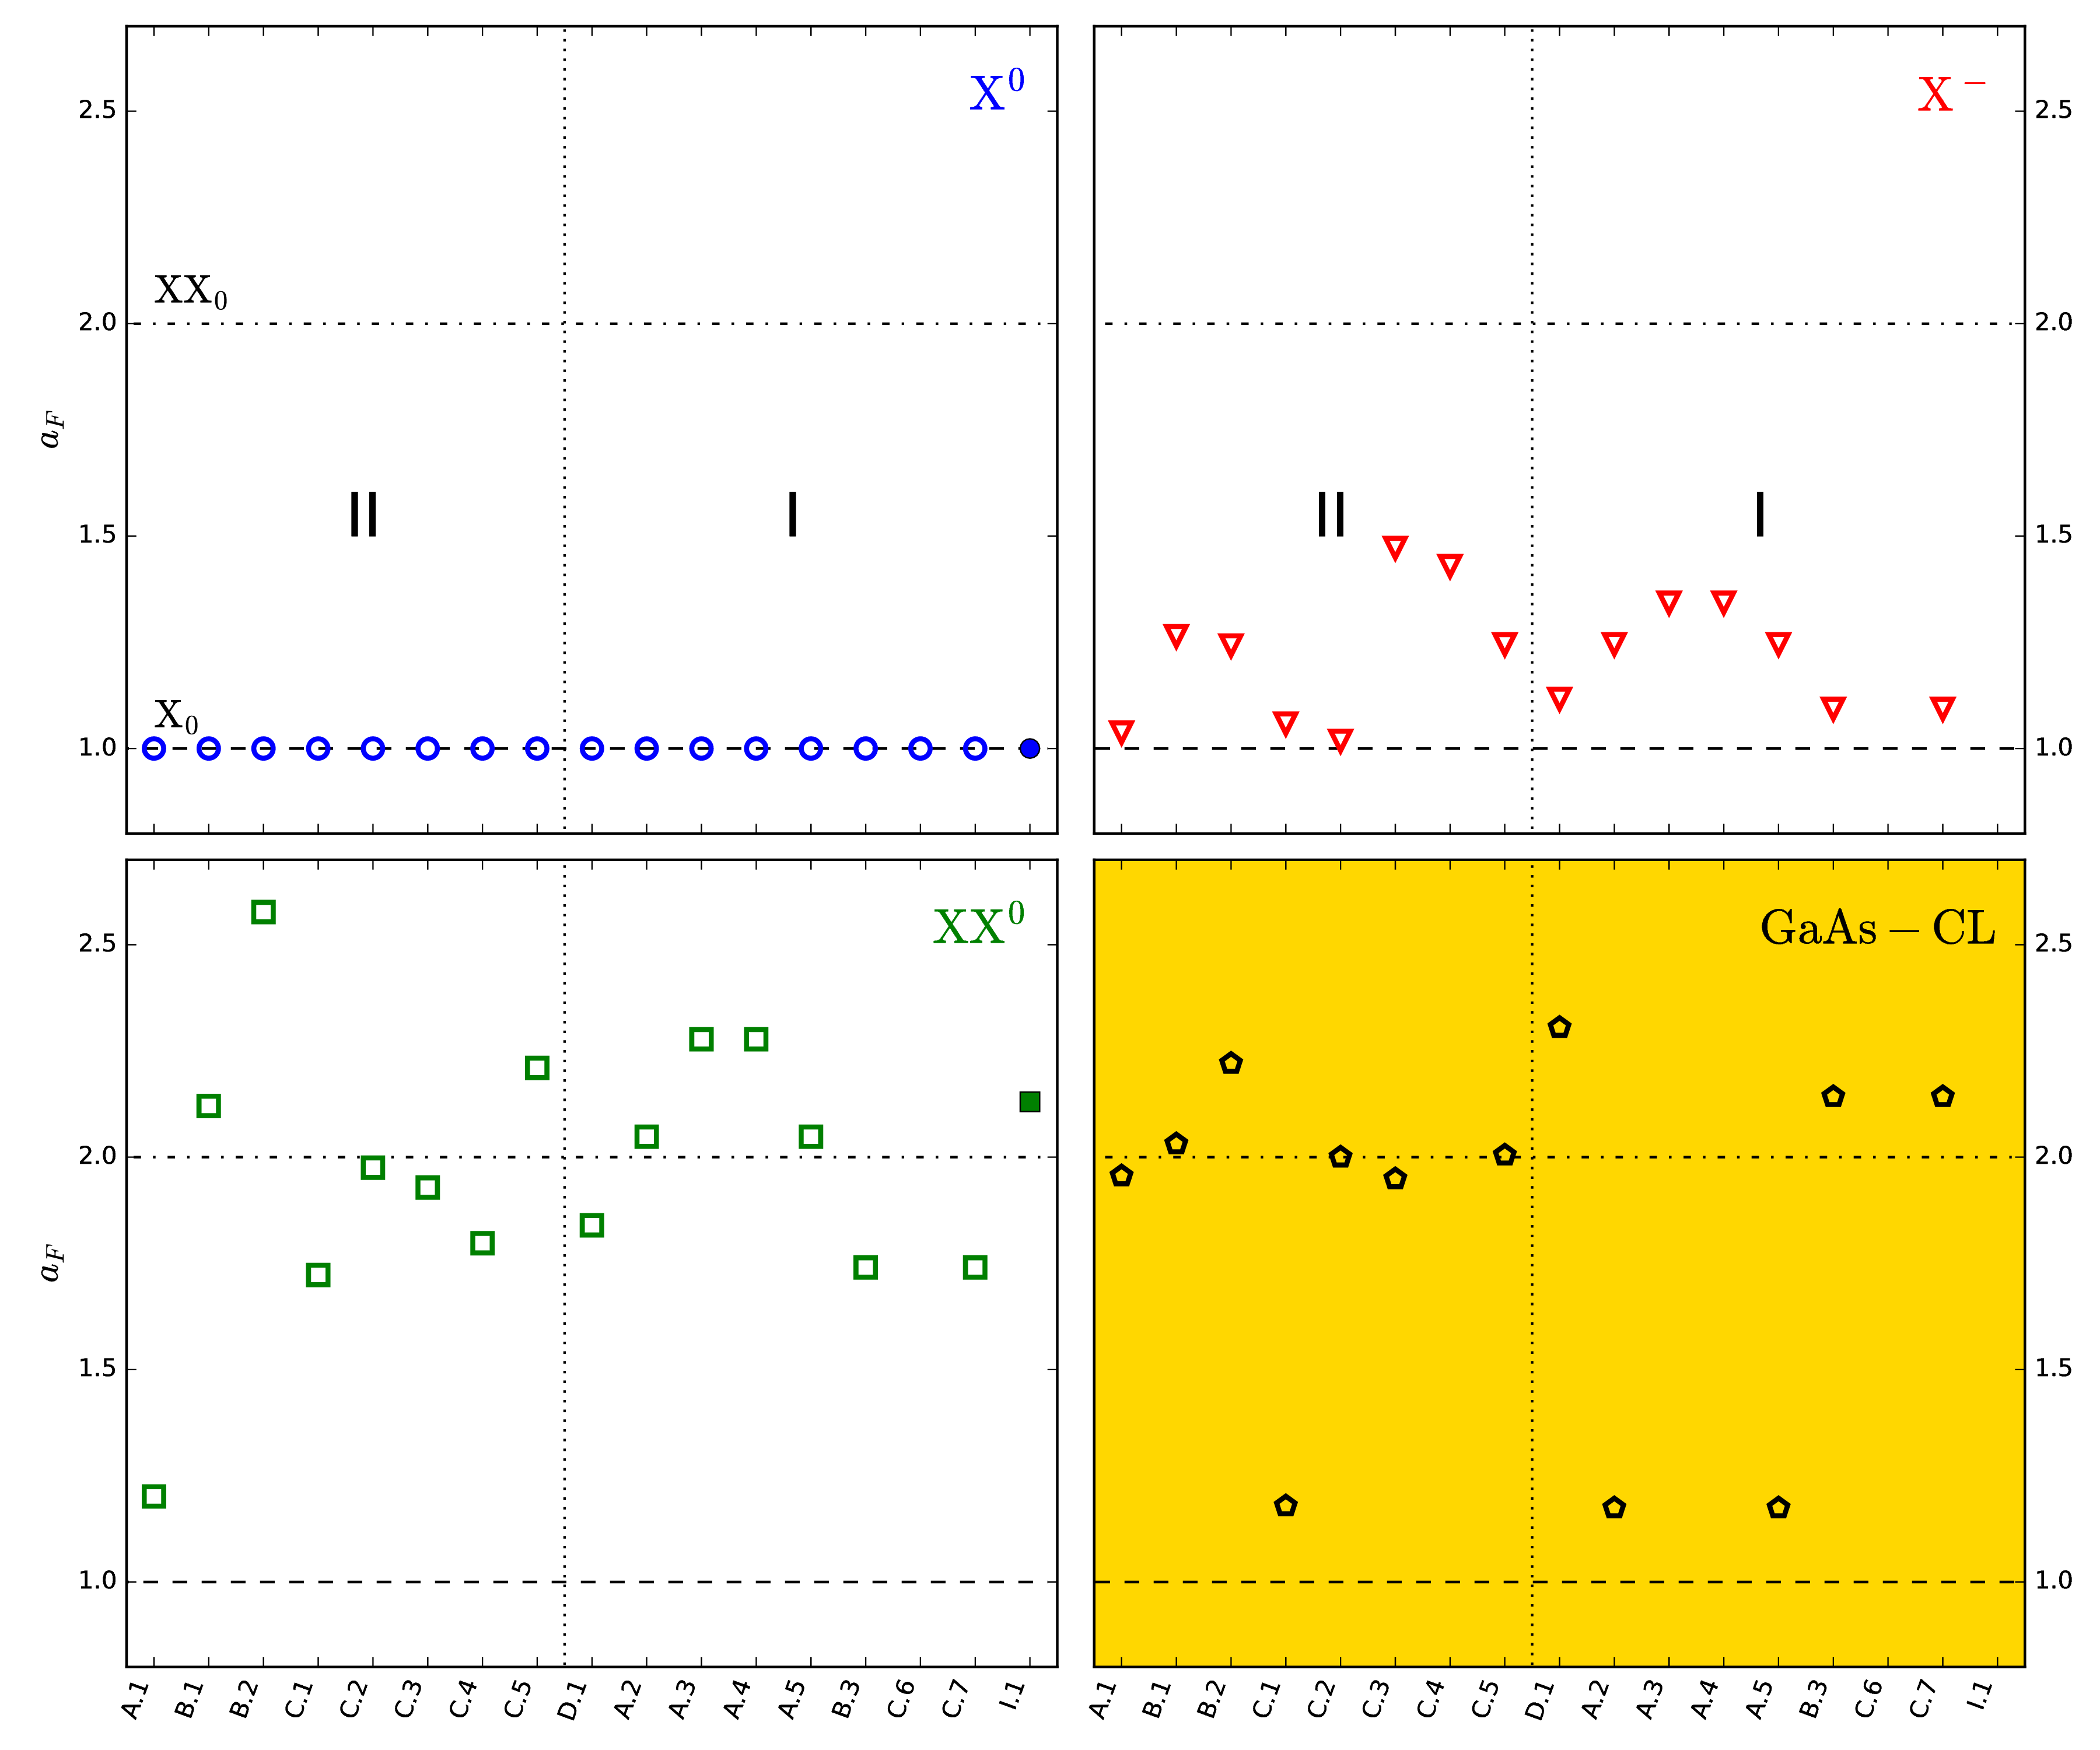
\includegraphics[width=0.7\linewidth]{/Sci_rep/suplament/osc}
	\caption{Summary of slopes $a_F$ of the linear fit of $F(P)$ for $X^0$ (blue circles), $X^-$ (red triangles), $XX^0$ (green squares), and that for the transition between bulk GaAs and CL (black pentagons). The data are shown for four samples with InGaAs/GaAsSb/GaAs QDs, marked as A through D on the horizontal axis and the sample with InAs/GaAs QDs marked by I; different numbers correspond to a different position on the corresponding sample. The slopes $a_F$ were normalized so that $a_F=1$ for $X^0$. The dotted vertical line divides QDs corresponding to type-II and type-I confinement, respectively. The horizontal lines mark the values of the slopes for free non-interacting exciton (dashed) and free non-interacting biexciton (dotted).}
	\label{fig:sup:osc_slope}
\end{figure}




\begin{figure}
	\centering
	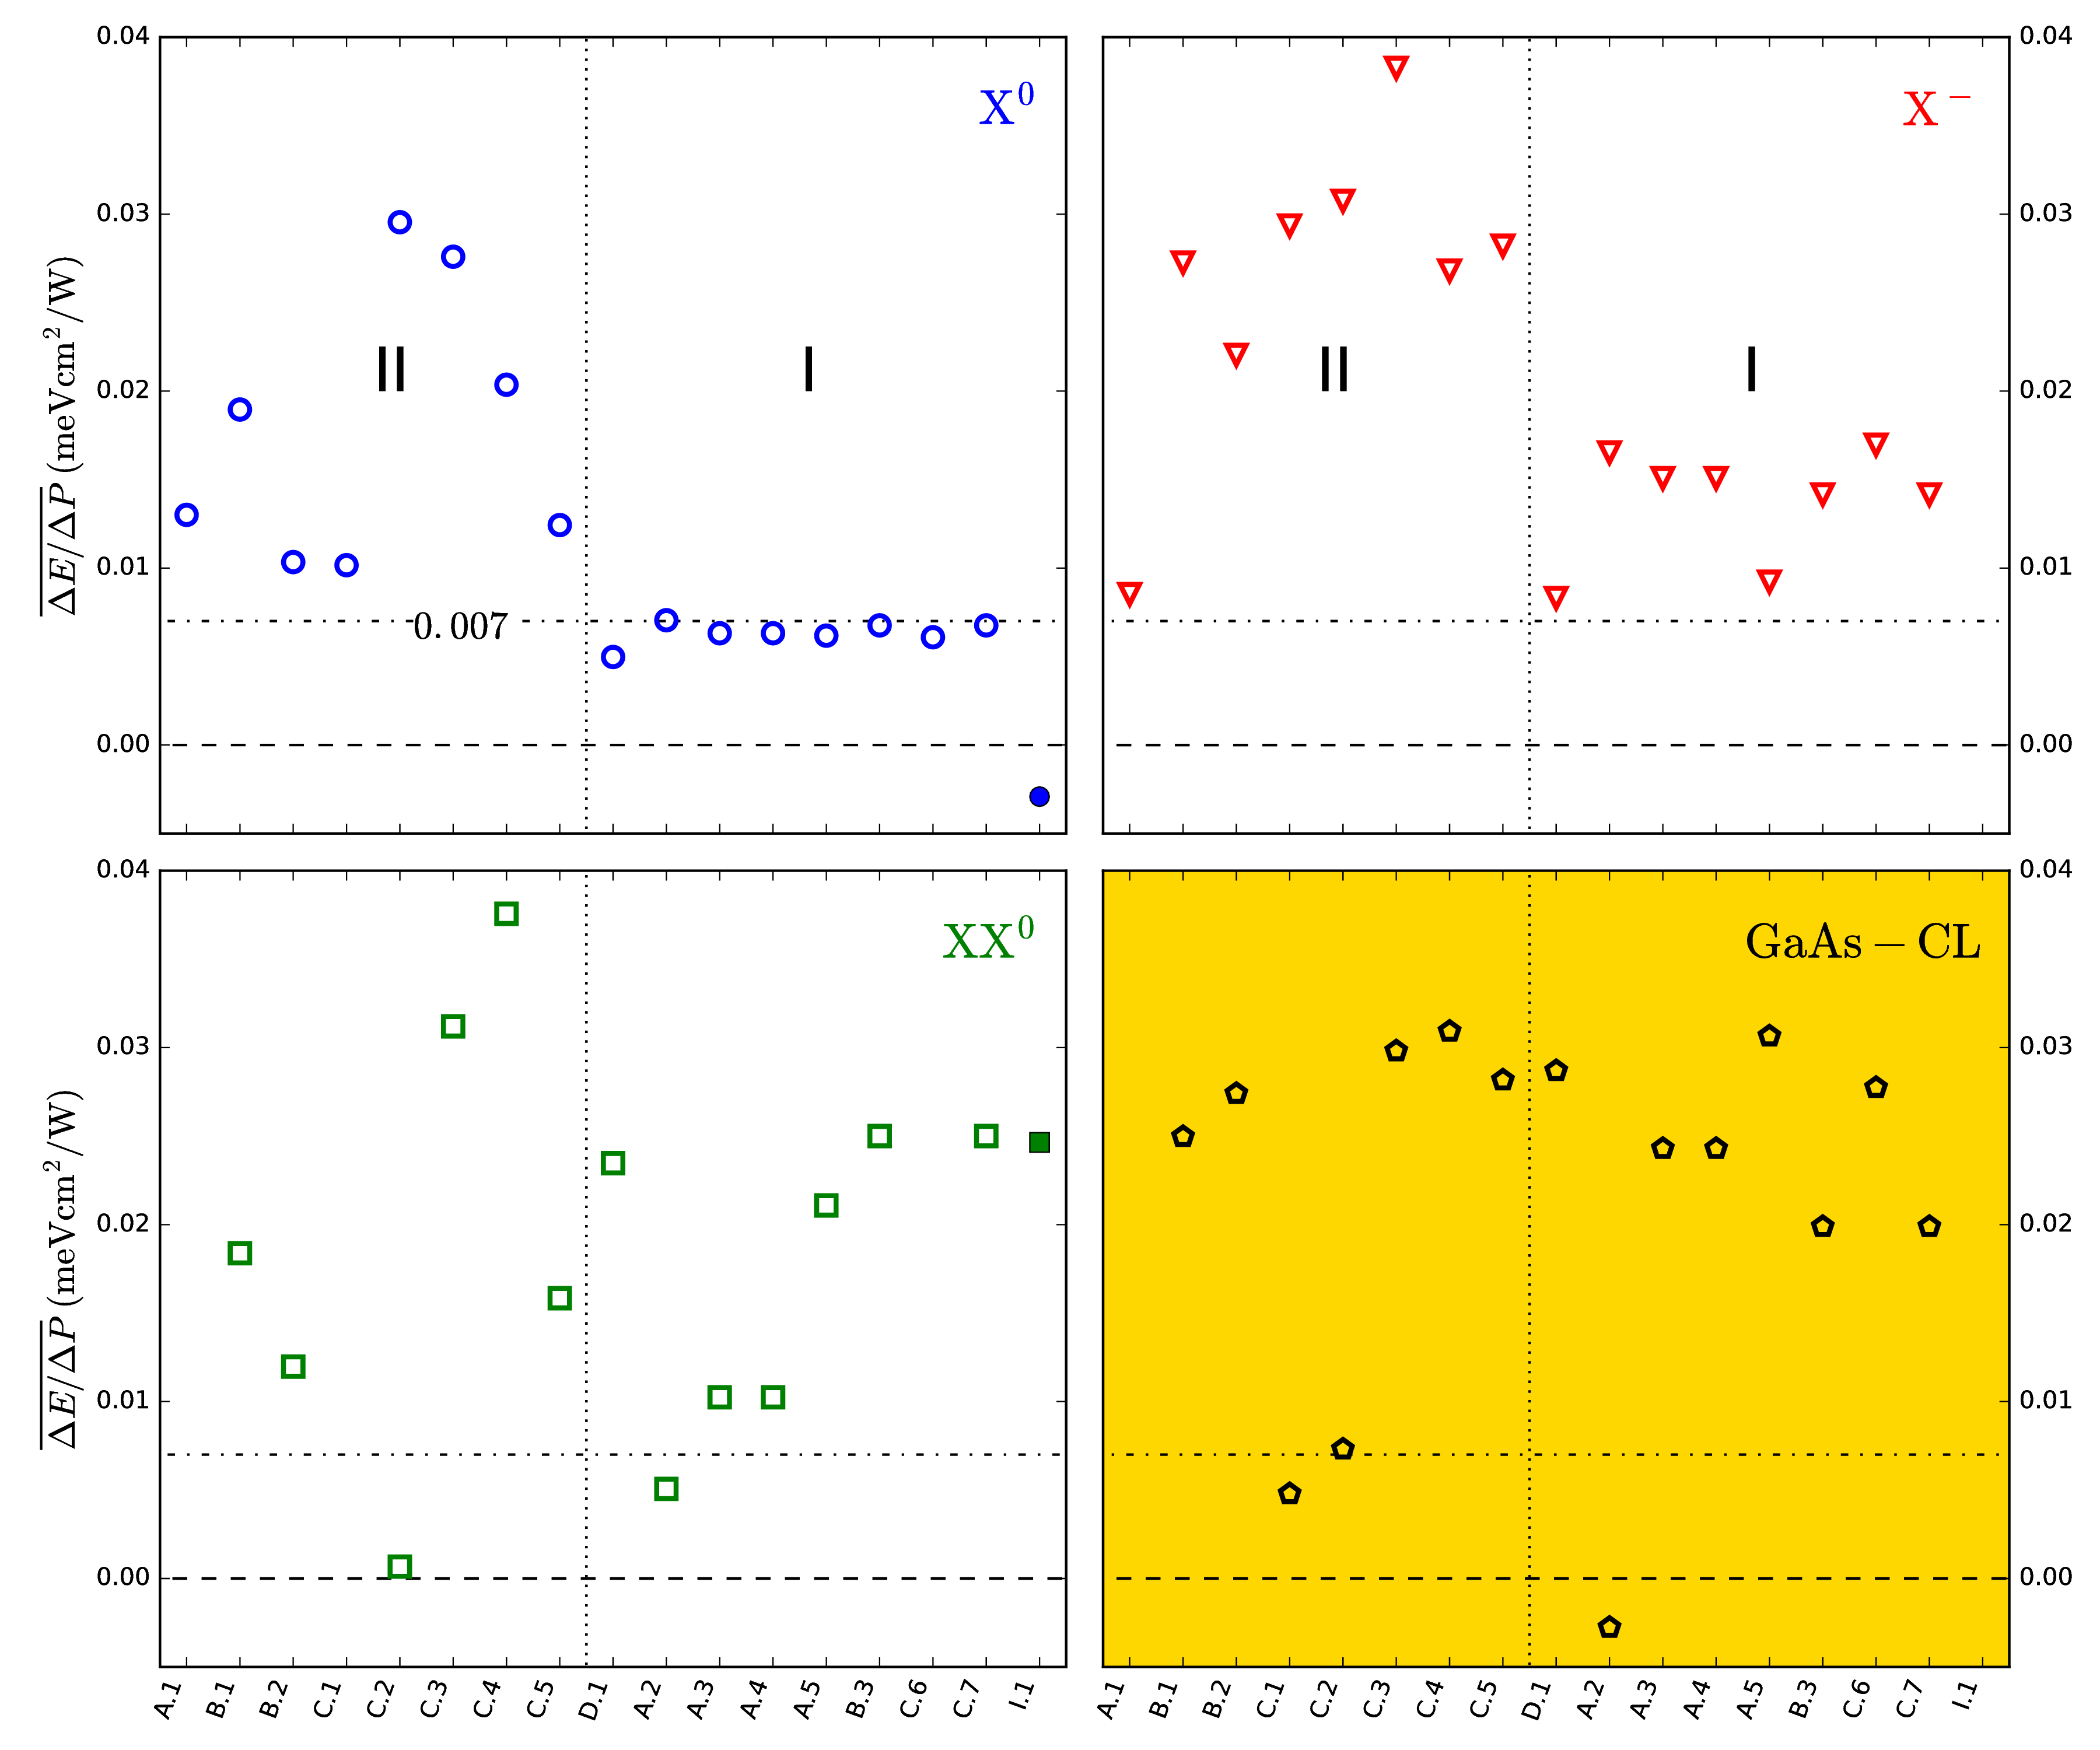
\includegraphics[width=0.7\linewidth]{/Sci_rep/suplament/mean_shift}
	\caption{Summary of the mean blue-shifts $\overline{\Delta E/\Delta P}$. The marking of the data is the same as in Fig.~\ref{fig:sup:osc_slope} except for the broken horizontal line marking zero value and the dashed horizontal one marking energy shift of $\overline{\Delta E/\Delta P}=0.007$ according to which we distribute the QD samples to those having type-I (or q-type-I) confinement and those presenting with type-II transition, respectively.}
	\label{fig:sup:mean_blueshift}
\end{figure}

\begin{figure}
	\centering
	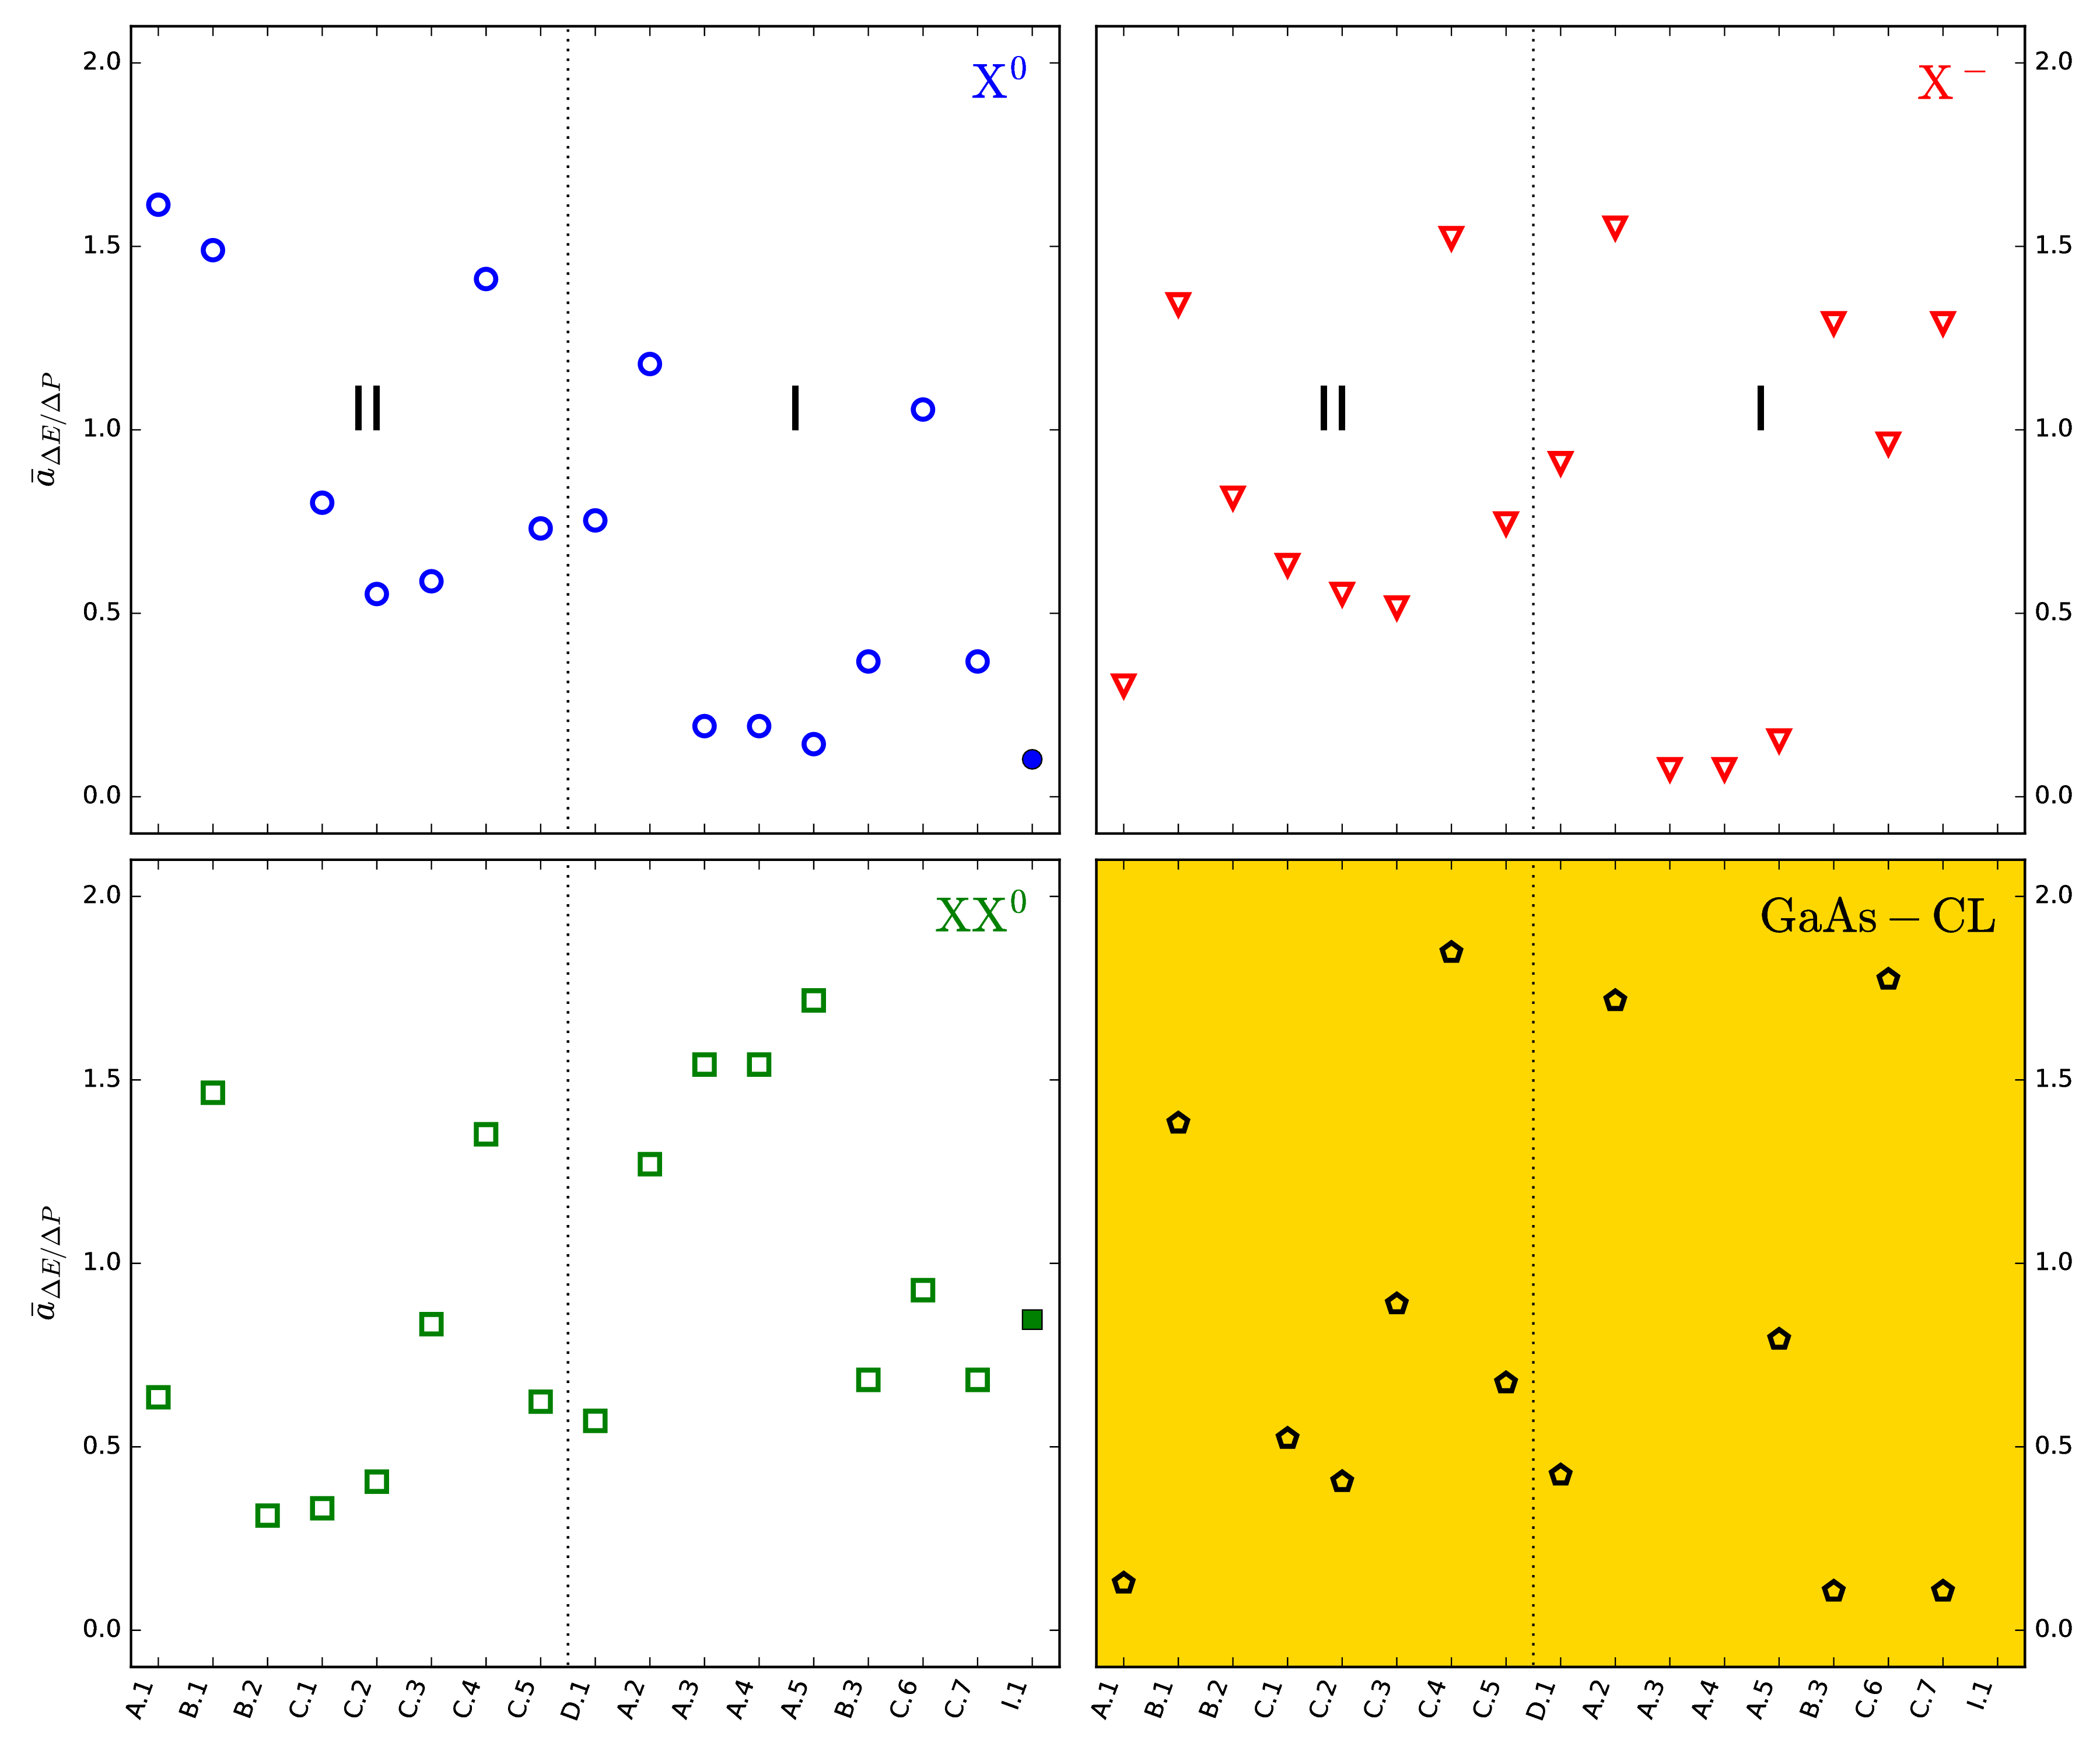
\includegraphics[width=0.7\linewidth]{/Sci_rep/suplament/blue-shift}
	\caption{Summary of the mean exponents $\bar{a}_{\Delta E/\Delta P}$ of $\Delta E\propto P^a$ dependence used for fitting of the $E(P)$ data. The marking is the same as in Fig.~\ref{fig:sup:mean_a_blueshift}.}
	\label{fig:sup:mean_a_blueshift}
\end{figure}



\begin{figure}
	\centering
	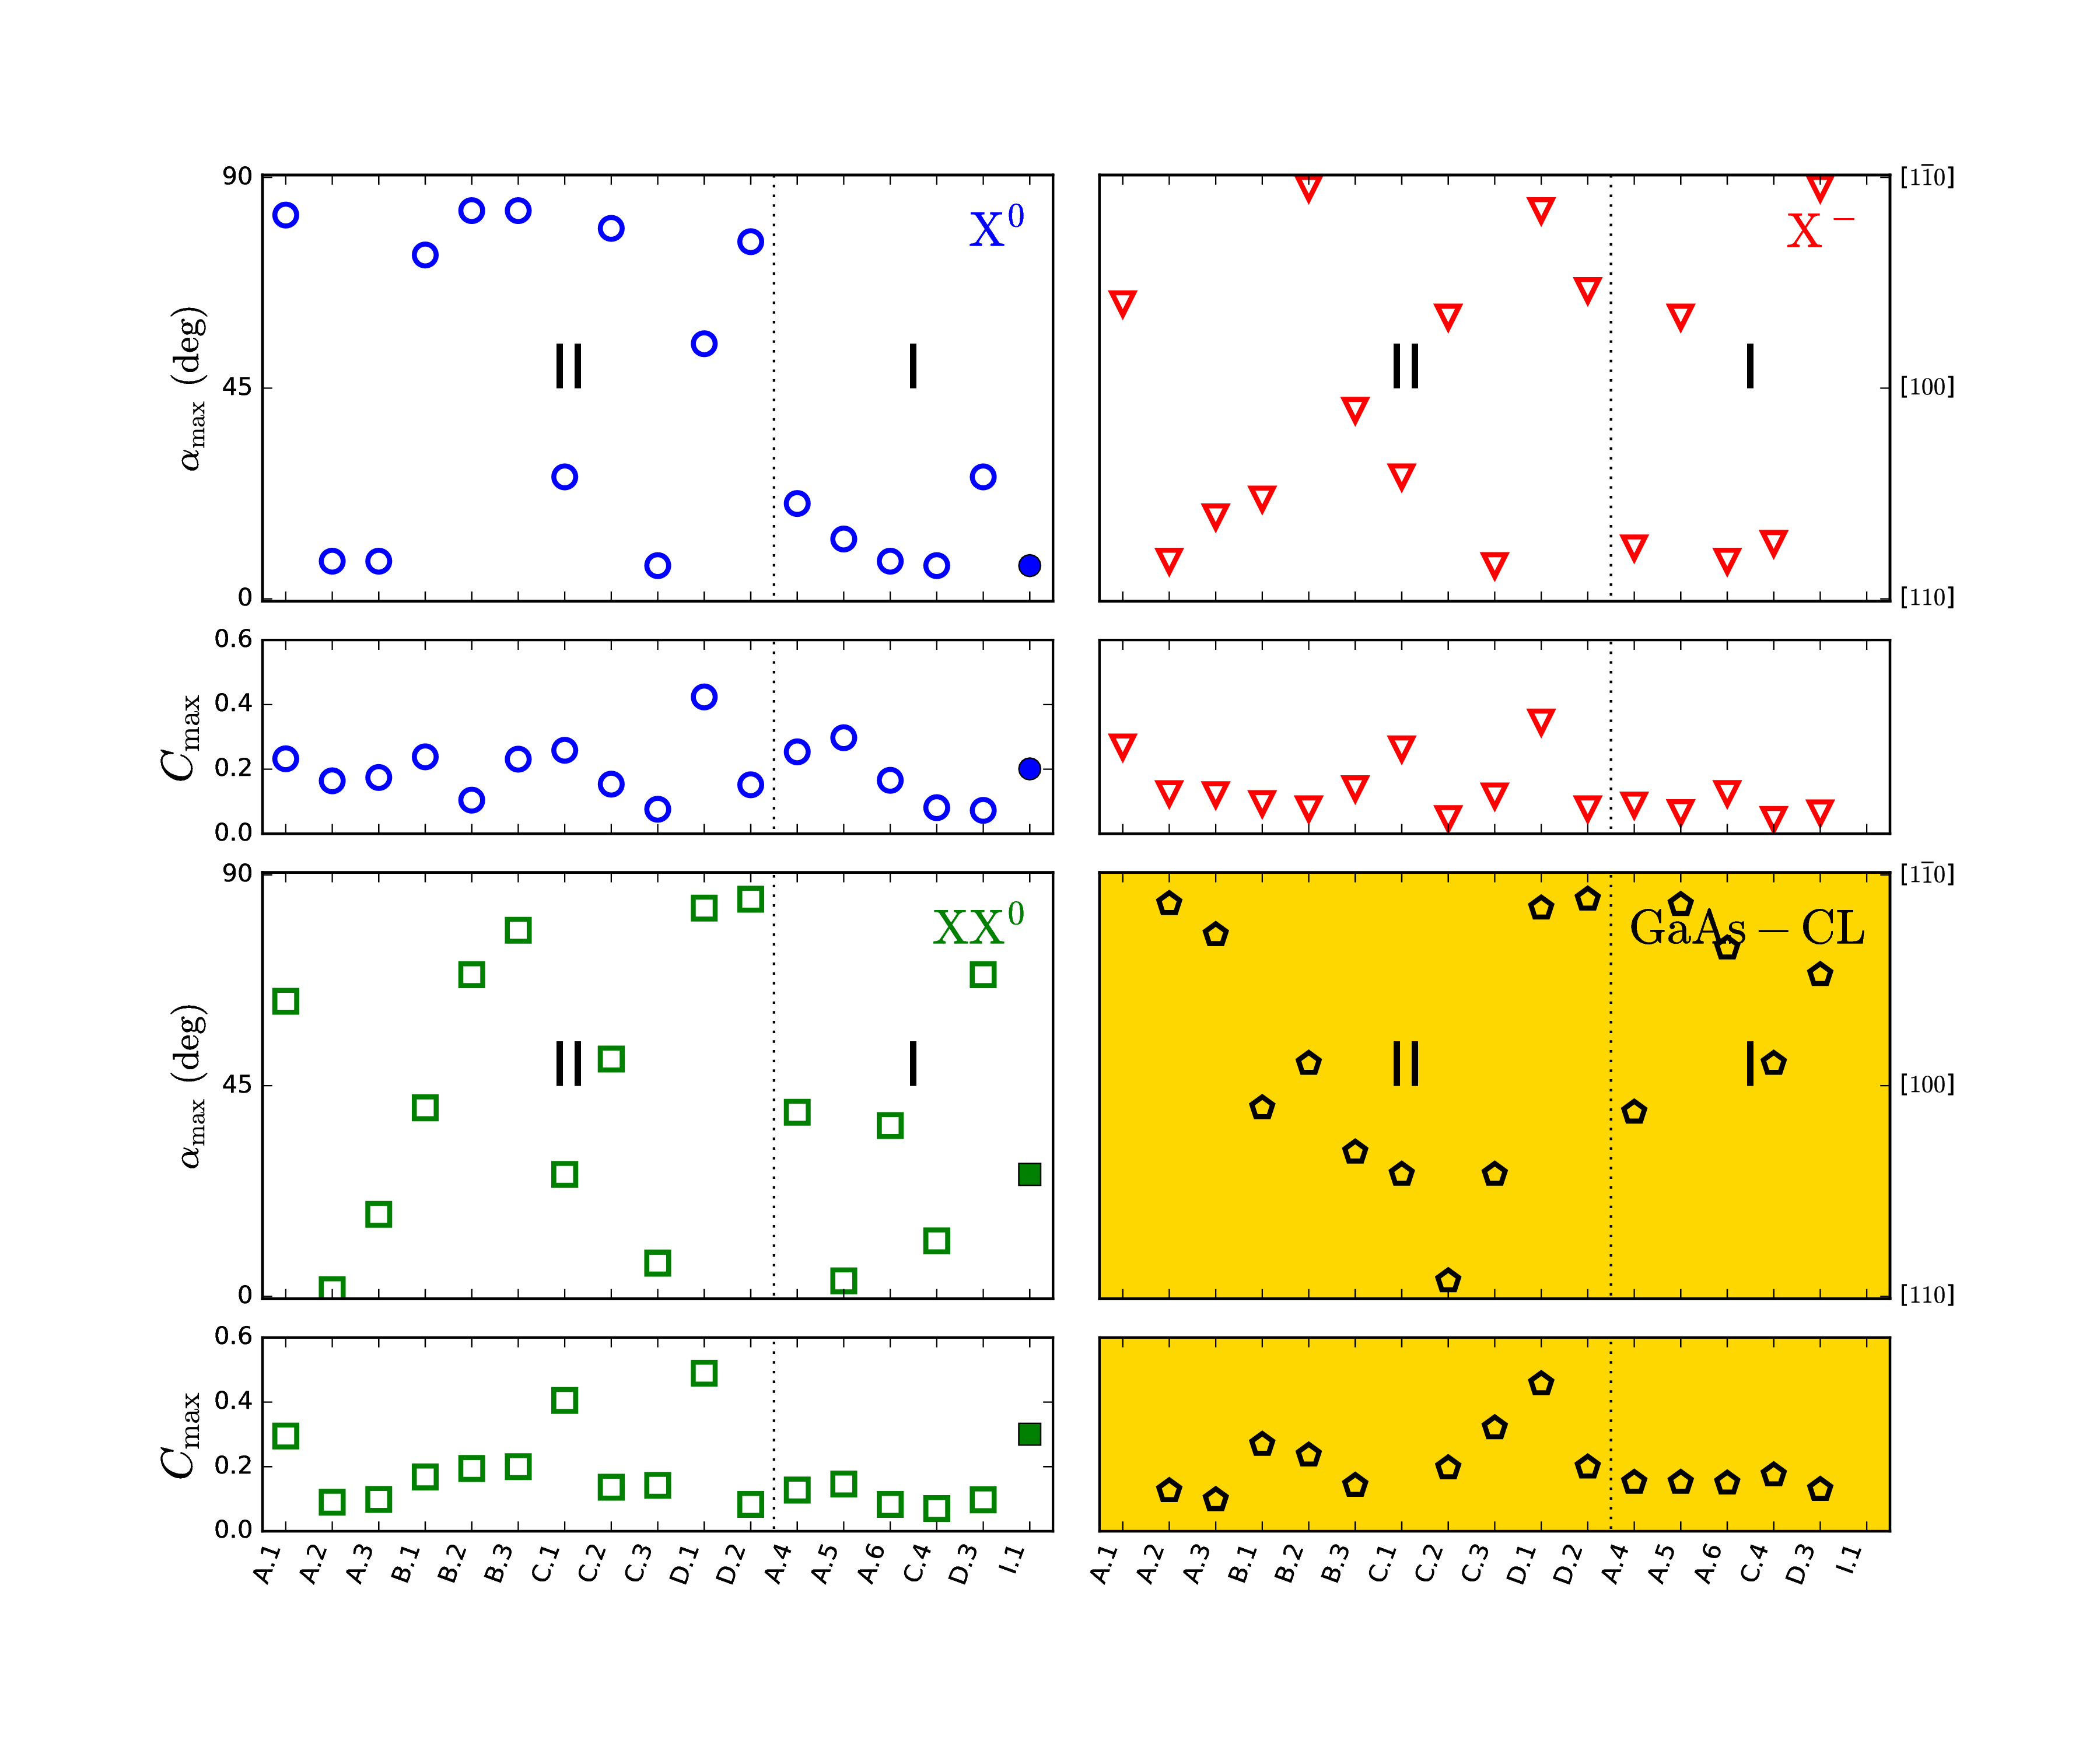
\includegraphics[width=0.7\linewidth]{/Sci_rep/suplament/polar}
	\caption{Summary of the azimuth $\alpha_{\mathrm{max}}$ and degree $C_{\mathrm{max}}$ of the polarization anisotropy of the multi-particle bands. The marking of the data is the same as in Figs.~\ref{fig:sup:osc_slope}. For each complex the upper panel corresponds to $\alpha_{\mathrm{max}}$ and the lower one to $C_{\mathrm{max}}$.}
	\label{fig:sup:pol}
\end{figure}
\newpage 